\lfoot{Autor: Daniel Melichar}
\subsubsection{Datenbankmanagementsysteme}
\label{subsec:dbms}

In der folgenden Sektion werden die gängisten RDBMS und NoSQL Datenbanken vorgestellt und gegeneinander vergleicht. Der Fokus liegt auf NoSQL-DBs, da diese in diesem Projekt verwendet werden.

\paragraph{Relationale DBMS}\mbox{}\\
\textbf{MySQL\newline}
Dieses RDBMS wurde ursprünglich entwickelt als \textit{lightweight database-like engine} und hatte in den ersten Versionen wenige von den Features die zu dem Zeitpunkt als essentiell gekennzeichnet waren. Trotz allem war es ein nützliches Tool, welches zwar kein eigentliches RDBMS, aber dennoch einfach zum Einrichten und Verwenden war.

In den letzten Jahren hat MySQL die Ziele der Applikation geändert – es hat sich zu einem kompletten RDBMS entwickelt.  Trotz Bekanntheit wird MySQL immer noch nicht als die stabilste Datenbank, oder jene mit dem größten Feature-Set, angesehen.

\textbf{Oracle\newline}
Dieses DBMS ist bekannt für seine große Anzahl an Features. Beinahe jedes Betriebssystem wird unterstützt; für die gängisten Programmierstellen gibt es Kommunikationsschnittstellen; es werden viele Server Programmiersprachen unterstützt hat viele Möglichkeiten; die Performance von Oracle Datenbanken ist exzellent; uvm.

\textbf{PostgreSQL\newline}
PostgreSQL, oder einfach nur Postgres, ist ein Open-Source Objekt relationales Datenbankmanagementsystem (ORDBMS). Es wird häufig für online Applikationen, Data Centers und für Domain Registrierung verwendet. PostgreSQL steht auch für viele Betriebssysteme zur Verfügung: Linux, Windows, FreeBSD, Solaris, etc.

\textbf{SQL Server\newline}
Microsoft's SQL Server wird in den meisten Fällen wird es für Webseiten, kommerzielle Applikationen und Netzwerk Applikationen verwendet. Der SQL Server verfügt über Features wie z.B. eine 10GB große Speicherkapazität für Datenbanken, \textit{safe-store} von Daten mit hohen Sicherheitsniveau, Data warehousing.\nextline 

In der folgenden Tabelle werden die System Eigenschaften der beschriebenen relationalen DBMS verglichen. Für eine genaue Übersicht bezüglich der unterstützten Features sollte folgende Website in Betracht gezogen werden \url{http://www.sql-workbench.net/dbms_comparison.html}

\begin{table}[!htb]
\centering
\label{rdbms-comp}
\resizebox{\columnwidth}{!}{%
\begin{tabular}{|l|l|l|l|l|}
\hline
\textbf{Name} & \multicolumn{1}{c|}{\textbf{Microsoft SQL Server}} & \textbf{MySQL} & \textbf{Oracle} & \textbf{PostgreSQL} \\ \hline
\textbf{Website} & www.microsoft.com/sqlserver & www.mysql.com & www.oracle.com/database & www.postgresql.org \\ \hline
\textbf{Developer} & Microsoft & Oracle & Oracle & \begin{tabular}[c]{@{}l@{}}PostgreSQL Global\\ Development Group\end{tabular} \\ \hline
\textbf{\begin{tabular}[c]{@{}l@{}}Erster \\ Release\end{tabular}} & 1989 & 1995 & 1980 & 1989 \\ \hline
\textbf{\begin{tabular}[c]{@{}l@{}}Momentaner \\ Release\end{tabular}} & \begin{tabular}[c]{@{}l@{}}SQL Server 2014\\ April 2014\end{tabular} & \begin{tabular}[c]{@{}l@{}}5.7.11\\ February 2016\end{tabular} & \begin{tabular}[c]{@{}l@{}}12 Release 1 (12.1.0.2)\\ July 2014\end{tabular} & \begin{tabular}[c]{@{}l@{}}9.5.1\\ February 2016\end{tabular} \\ \hline
\textbf{Lizenz} & Kommerziell & Open Source / Kommerziell & Kommerziell & Open Source \\ \hline
\textbf{\begin{tabular}[c]{@{}l@{}}Entwickelt\\ in..\end{tabular}} & C++ & C und C++ & C und C++ & C \\ \hline
\textbf{\begin{tabular}[c]{@{}l@{}}Unterstütze\\ Server\\ Systeme\end{tabular}} & Windows & \begin{tabular}[c]{@{}l@{}}FreeBSD\\ Linux\\ OS X\\ Solaris\\ Windows\end{tabular} & \begin{tabular}[c]{@{}l@{}}AIX\\ HP-UX\\ Linux\\ OS X\\ Solaris\\ Windows\\ z/OS\end{tabular} & \begin{tabular}[c]{@{}l@{}}FreeBSD\\ HP-UX\\ Linux\\ NetBSD\\ OpenBSD\\ OS X\\ Solaris\\ Unix\\ Windows\end{tabular} \\ \hline
\textbf{\begin{tabular}[c]{@{}l@{}}Unterstütze\\ Sprachen\end{tabular}} & \begin{tabular}[c]{@{}l@{}}.NET\\ Java\\ PHP\\ Python\\ Ruby\\ Visual Basic\end{tabular} & \begin{tabular}[c]{@{}l@{}}Ada\\ C\\ C\#\\ C++\\ D\\ Eiffel\\ Erlang\\ Haskell\\ Java\\ Objective-C\\ OCaml\\ Perl\\ PHP\\ Python\\ Ruby\\ Scheme\\ Tcl\end{tabular} & \begin{tabular}[c]{@{}l@{}}C\\ C\#\\ C++\\ Clojure\\ Cobol\\ Eiffel\\ Erlang\\ Fortan\\ Groovy\\ Haskell\\ Java\\ JavaScript\\ Lisp\\ Objective-C\\ OCaml\\ Perl\\ PHP\\ Python\\ R\\ Ruby\\ Scala\\ Tc\\ Visual Basic\end{tabular} & \begin{tabular}[c]{@{}l@{}}.NET\\ C\\ C++\\ Java\\ Perl\\ Python\\ Tcl\end{tabular} \\ \hline
\textbf{\begin{tabular}[c]{@{}l@{}}APIs und \\ andere Verbindungs-\\ möglichkeiten\end{tabular}} & \begin{tabular}[c]{@{}l@{}}OLE DB\\ Tabular Data Stream (TDS)\\ ADO.NET\\ JDBC\\ ODBC\end{tabular} & \begin{tabular}[c]{@{}l@{}}ADO.NET\\ JDBC\\ ODBC\end{tabular} & \begin{tabular}[c]{@{}l@{}}ODP.NET\\ Oracle Call Interface (OCI)\\ JDBC\\ ODBC\end{tabular} & \begin{tabular}[c]{@{}l@{}}Native C Libary\\ ADO.NET\\ JDBC\\ ODBC\end{tabular} \\ \hline
\end{tabular}
}
\caption{Vergleich von relationalen Datenbankmanagementsystemen \cite{MELD.CH2-dbms.compRDBMS}}
\end{table}

\clearpage

\paragraph{NoSQL Datenbanken}\mbox{}\\

Grundsätzlich gibt es vier große Gruppen von NoSQL Datenbanken \cite{MELD.CH2-dbms.compNoSQLInfo}: Key-Value Stores, Column-Oriented Databases, Document Databases und Graph Stores. Selbstverständlich gibt es auch eigens entwickelte Datenbanken die nicht in diese vier Kategorien eingeteilt werden können, diese vier sind aber jene die am meisten verwendet werden \cite{MELD.CH2-dbms.compNoSQLInfo}.

\begin{itemize}
	\item \textbf{Key-Value Stores\newline}
	In einem Key-Value Store werden Daten in Form von eindeutigen Schlüsseln (Keys) und damit verknüpften Werten (Values) gespeichert (siehe Abbildung \ref{fig:keyvalue}). Diese Art von Datenbank ist prinzipiell ziemlich simple, aber dennoch effizient und schnell. In den meisten Fällen findet die Kommunikation mit der Datenbank mittels einer API, die für mehrere Programmiersprachen zur Verfügung gestellt wurde, statt und der Key mittels Strings realisiert welche dann auf die Values (also die eigentlichen Daten) referenzieren. Diese Datenbanken sind Hash-Tabellen sehr ähnlich, da auch hier der Key als Index verwendet wird und somit schnelle Zugriffszeiten ermöglicht werden. Wie bei den meisten NoSQL Datenbanken ist auch bei Key-Value kein Schema aufzufinden.

	Beispielhafte Anwendungen von Key-Value Datenbaken wären die Speicherung von Session Daten eines Users, die Speicherung der Artikel in einem Einkaufswagen, oder die Speicherung der beliebten Produkte.

	Bekannte Key-Value Datenbanken: Amazon DynamoDB und RIAK\nextline

	\begin{figure}[h]\centering
		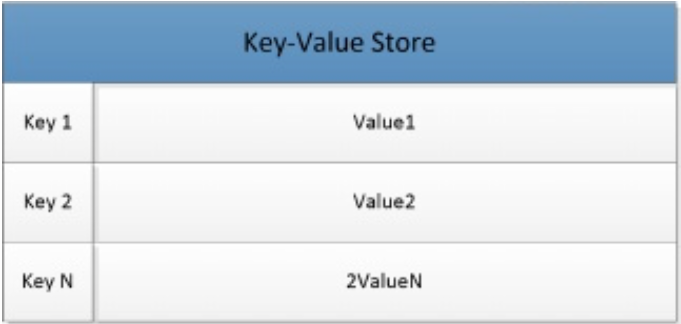
\includegraphics[width=0.5\textwidth]{images/keyvalueStore}
		\caption{Aufbau von Key-Value Datenbanken}
		\label{fig:keyvalue}
	\end{figure}

	\item \textbf{Column-Oriented Databases\newline}
	Relationale DBMS speichern die Daten in Form von Zeilen, bei Column Stores werden diese in Zellen gespeichert (siehe Abbildung \ref{fig:columnstore}). Es herrscht zwar das selbe Konzept der Abspeicherung mehrerer Objekte mit einer Referenz auf die selbe ID, wie bei relationalen Datenbanken, aber diese werden nicht in Tabellen gespeichert, sondern in massiven, verteilten Architekturen. Jeder Key ist mit einer oder mehreren Attributen verknüpft. Diese Art von Datenbank ist grundsätzlich so aufgebaut das mit einem einzigen Befehl eine große Menge an Daten zurückgebracht werden kann. 

	Column Store Datenbanken werden sehr oft für Data Mining, Datawarehousing und im Allgemeinen für Business Analytics verwendet.

	Einige der Bekanntesten Datenbanken sind: Googe BigTable, Cassandra

	\begin{figure}[h]\centering
		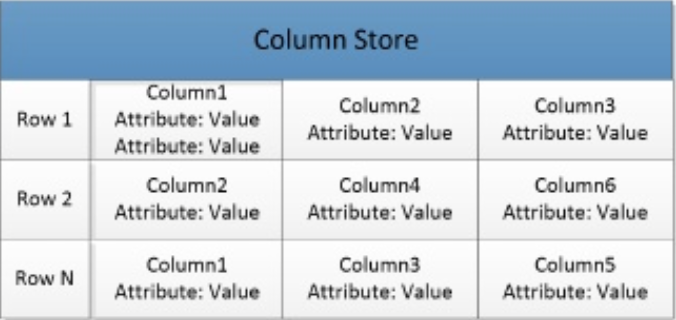
\includegraphics[width=0.5\textwidth]{images/columnStore}
		\caption{Aufbau von Column-Oriented Datenbanken}
		\label{fig:columnstore}
	\end{figure}


	\item \textbf{Document Databases\newline}
	Document Store Datenbanken sind jene Datenbanken bei welchen die Daten mittels einer quasi strukturiereten Datei gespeichert werden (siehe Abbildung \ref{ig:documentdb}). Oft werden sturkturen wie JSON, CSV, oder XML verwendet. Intern werden die Daten dann mittels der bereits bekannten Key-Value Methodik gespeichert - der einzige Unterschied liegt also in der Verarbeitungweise der Anfragen des Users. Hierbei ist vor allem auf die Performance und horizontale Skalierbarkeit zu achten. Die Files, oder Dokumente, in einer Document-Oriented Datenbank sind ähnlich zu jenen einer relationalen Datenbank, aber der große Unterschied hierbei ist, dass diese an kein Schema gebunden und somit um einiges flexibler sind. Diese Dokumente sind mittels einem eindeutigen Key adressiert, welcher das File auch repräsentiert. Diese Keys können einfache Strings oder ganze Pfade sein.

	Anwendungsgebiete von dieser Art von Datenbank sind Applikationen wie Content Management Systeme, Blog Software, usw. 

	Die bekanntesten Document-oriented Datenbanken sind: MongoDB und CouchDB

	\begin{figure}[h]\centering
		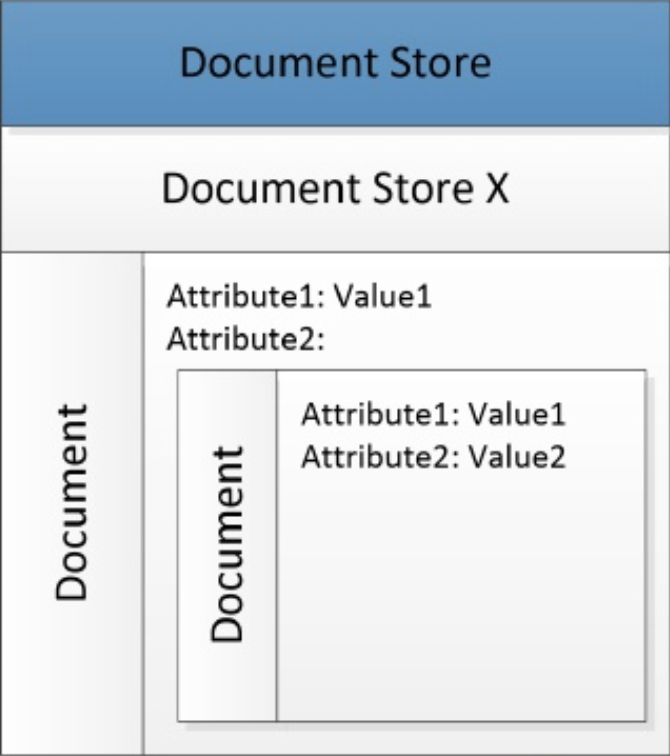
\includegraphics[width=0.3\textwidth]{images/documentStore}
		\caption{Aufbau von Document Datenbanken}
		\label{fig:documentdb}
	\end{figure}

	\clearpage

	\item \textbf{Graph Stores\newline}
	In Graph Datenbanken werden die Daten mittels so genannten Nodes und Edges gespeichert, wobei Nodes als Objekte arbeiten und Edges die Beziehungen zwischen den einzelnen Objekten (siehe Abbildung \ref{fig:graphdb}). Es wird hier die \textit{Index-Free-Adjacency} Technik verwendet. Das bedeutet, dass jeder Node mit Pointern versetzt wurde die es ermöglichen auf den nächstgelegenen Node Zugriff zu bekommen. Somit kann mit einem Befehl über mehrere Nodes iteriert werden. In Graph-Oriented Datenbanken liegt der Hauptsächliche Fokus auf die Verbindung zwischen den Daten, also in welcher Beziehung diese stehen. Anders als bei anderen NoSQL Datenbanken werden bei Graph Datenbanken oftmals Teile des ACID Models verwendet.

	Sozialle Netzwerke sind die hauptsächlichen Anwendungsgebiete von Graph Datenbanken, aber auch Applikationen für Sicherheits- und Zugriffskontrollen, Content Management Systeme, Cloud Management, etc. 

	Ein verbreiteter Vertreter dieser Kategorie ist Neo4J.

	\begin{figure}[h]\centering
		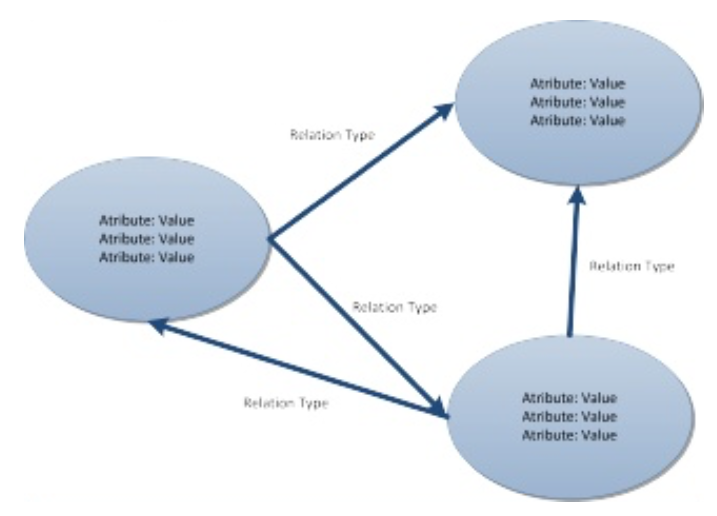
\includegraphics[width=0.5\textwidth]{images/graphStore}
		\caption{Aufbau von Graph Datenbanken}
		\label{fig:graphdb}
	\end{figure}
\end{itemize}
\clearpage

Hier kann man nochmals jene NoSQL Datenbanken betrachten und vergleichen die zum haufigsten Zeitpunkt am meisten verwendet werden.

\begin{figure}[!htb]\centering
	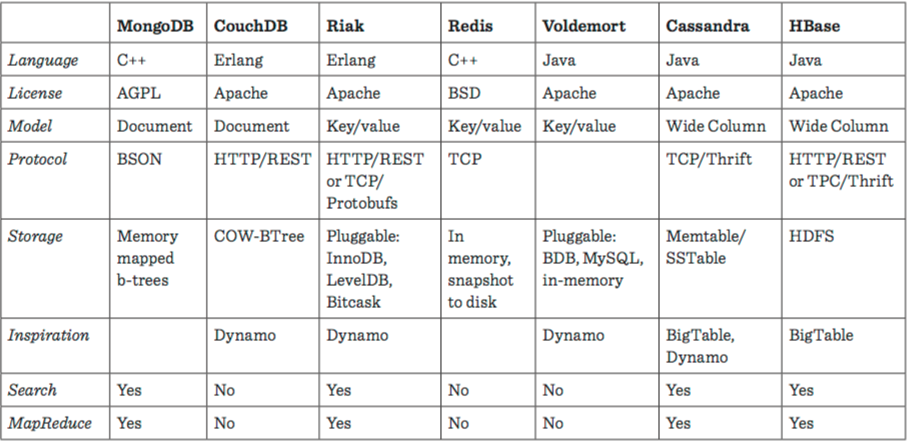
\includegraphics[width=1\textwidth]{images/noSQLComp}
	\caption{Vergleich von gängigen NoSQL Datenbanken\cite{MELD.CH2-dbms.compNoSQL}}
\end{figure}


\clearpage % DO NOT REMOVE